\documentclass[12pt, a4paper]{report}
\usepackage[utf8]{inputenc}
\usepackage[T1]{fontenc}
\usepackage{graphicx}
\usepackage{booktabs}
\usepackage{caption}
\usepackage{fancyhdr}
\usepackage{geometry}
\geometry{a4paper, margin=1in}
\usepackage{tikz}
\usetikzlibrary{matrix, positioning, arrows.meta}
\usepackage{xcolor}
\usepackage{fontawesome5}
\usepackage{hyperref}
\usepackage{tcolorbox}
\usepackage{needspace}
\usepackage{float}            % for [H] table placement
\usepackage{enumitem}         % better list spacing
\usepackage{microtype}        % improves typography
\usepackage{titlesec}         % custom title formatting
\usepackage{colortbl}         % moved here to prevent empty first page
\tcbuselibrary{skins,breakable}

% -------------------------------------------------------------
% Color palette (navy, teal, gold, light backgrounds)
% -------------------------------------------------------------
\definecolor{navy}{RGB}{12, 35, 70}
\definecolor{teal}{RGB}{20, 120, 110}
\definecolor{gold}{RGB}{210, 170, 80}
\definecolor{lightbg}{RGB}{245, 248, 250}
\definecolor{codebg}{RGB}{240, 245, 245}

% Hyperlink colors
\hypersetup{
    colorlinks=true,
    linkcolor=teal,
    citecolor=teal,
    urlcolor=teal,
    pdfauthor={Ons Aissa, Ranime Gharbi},
    pdftitle={DataCo Smart Supply Chain Analytics}
}

% -------------------------------------------------------------
% Color hierarchy for chapters, sections, subsections
% -------------------------------------------------------------
\titleformat{\chapter}
  {\normalfont\Huge\bfseries\color{navy}}{\thechapter}{20pt}{}
\titlespacing*{\chapter}{0pt}{-20pt}{40pt}
\titleformat{\section}
  {\normalfont\Large\bfseries\color{teal}}{\thesection}{1em}{}
\titleformat{\subsection}
  {\normalfont\large\bfseries\color{navy}}{\thesubsection}{1em}{}
\titleformat{\subsubsection}
  {\normalfont\normalsize\bfseries\color{gold}}{\thesubsubsection}{1em}{}

% Add a subtle rule below chapter titles
\titleformat{\chapter}
  {\normalfont\Huge\bfseries\color{navy}}{\thechapter}{20pt}{}
  [\vspace{0.3cm}\titlerule]

% -------------------------------------------------------------
% Header / footer
% -------------------------------------------------------------
\pagestyle{fancy}
\fancyhf{}
\fancyhead[R]{\nouppercase{\leftmark}}
\fancyfoot[C]{\thepage}
\renewcommand{\headrulewidth}{0.4pt}
\renewcommand{\chaptermark}[1]{\markboth{#1}{}}

\fancypagestyle{plain}{%
   \fancyhf{}
   \fancyhead[R]{\nouppercase{\leftmark}}
   \fancyfoot[C]{\thepage}
   \renewcommand{\headrulewidth}{0.4pt}
}

\fancypagestyle{empty}{%
   \fancyhf{}
   \renewcommand{\headrulewidth}{0pt}
}

% -------------------------------------------------------------
% Custom boxes for code and notes
% -------------------------------------------------------------
\newtcolorbox{codebox}{colback=codebg, colframe=teal, boxrule=1pt, arc=4pt, left=6pt, right=6pt, top=6pt, bottom=6pt, fonttitle=\bfseries\color{navy}, title=Code Snippet}
\newtcolorbox{infobox}{colback=lightbg, colframe=gold, boxrule=1pt, arc=4pt, left=6pt, right=6pt, top=6pt, bottom=6pt, fonttitle=\bfseries\color{navy}, title=Note}

% -------------------------------------------------------------
% \rowcolors removed from preamble — applied locally per table via \altrows
% -------------------------------------------------------------
\newcommand{\altrows}{\rowcolors{2}{lightbg}{white}}
\setlength{\aboverulesep}{0pt}
\setlength{\belowrulesep}{0pt}
\captionsetup{skip=5pt}

% -------------------------------------------------------------
% Document begins
% -------------------------------------------------------------
\begin{document}

% ==========================
% Title page (logos side by side on the right, FST left, UTM right)
% ==========================
\begin{titlepage}
   \thispagestyle{empty}
   \begin{tikzpicture}[remember picture, overlay]
      \fill[lightbg] (current page.north west) rectangle (current page.south east);
      \fill[teal, opacity=0.08] (current page.north west) .. controls (2, -2) and (5, -1) .. (8, -3) .. controls (4, -5) and (0, -4) .. cycle;
      \fill[gold, opacity=0.08] (current page.south east) .. controls (-2, 2) and (-5, 1) .. (-8, 3) .. controls (-4, 5) and (0, 4) .. cycle;
      \draw[teal, opacity=0.2, line width=0.6pt] (current page.north west) ++(2cm, -3cm) -- ++(14cm, 0);
      \draw[gold, opacity=0.3, line width=0.6pt] (current page.south west) ++(2cm, 3cm) -- ++(14cm, 0);
   \end{tikzpicture}
   \vspace*{1cm}
   \begin{center}
      % Logos: both on the right side, FST left, UTM right (next to each other)
      \hfill
      \begin{minipage}{0.5\textwidth}
         \centering
         
\includegraphics[height=1.2cm]{fst_logo.png}\hspace{1cm}%
         
\includegraphics[height=1.2cm]{utm_logo.png}
      \end{minipage}
      \hfill\null
      
      \vspace{0.6cm}
      {\color{navy}\Large\bfseries University of Tunis El Manar (UTM)\par}
      {\color{navy}\large Faculty of Sciences of Tunis (FST)\par}
      \vspace{2.2cm}
      {\color{navy}\Huge\bfseries DataCo Smart Supply Chain Analytics\par}
      \vspace{0.5cm}
      {\color{teal}\Large Final Project Report\par}
      \vspace{1.8cm}
      {\color{navy}\large
      \begin{tabular}{@{}l@{}}
         \textbf{Team:} Ons AISSA \& Ranime GHARBI \\[0.2cm]
         \textbf{Professor:} Manel ZEKRI \\[0.2cm]
         \textbf{Level:} 1st year Data Science Engineering \\[0.2cm]
         \textbf{Academic Year:} 2025–2026
      \end{tabular}
      \par}
      \vspace{2.2cm}
      {\color{teal}\Huge
         \faPython \hspace{0.8cm}
         \faFire \hspace{0.8cm}
         \faDatabase \hspace{0.8cm}
         \faChartLine \hspace{0.8cm}
         \faRobot \hspace{0.8cm}
         \faRandom
      }
      \vfill
   \end{center}
\end{titlepage}

% ==========================
% Table of Contents
% ==========================
\thispagestyle{empty}
\tableofcontents
\clearpage

% ==========================
% Main content
% ==========================

\chapter{Introduction}
\section{What is a supply chain?}
A supply chain is the \textbf{series of steps} that brings a product from its raw materials to the customer's hands.  
Imagine a chocolate bar: cocoa beans are grown on a farm, then transported to a factory where they are roasted and mixed with sugar and milk, then packaged, then shipped to a supermarket, and finally bought by you. Each step involves different people, companies, and vehicles. The "supply chain" is the whole system that makes this happen – and makes sure the right product arrives at the right place, at the right time, in the right condition, and at the right cost.

\begin{figure}[H]
   \centering
   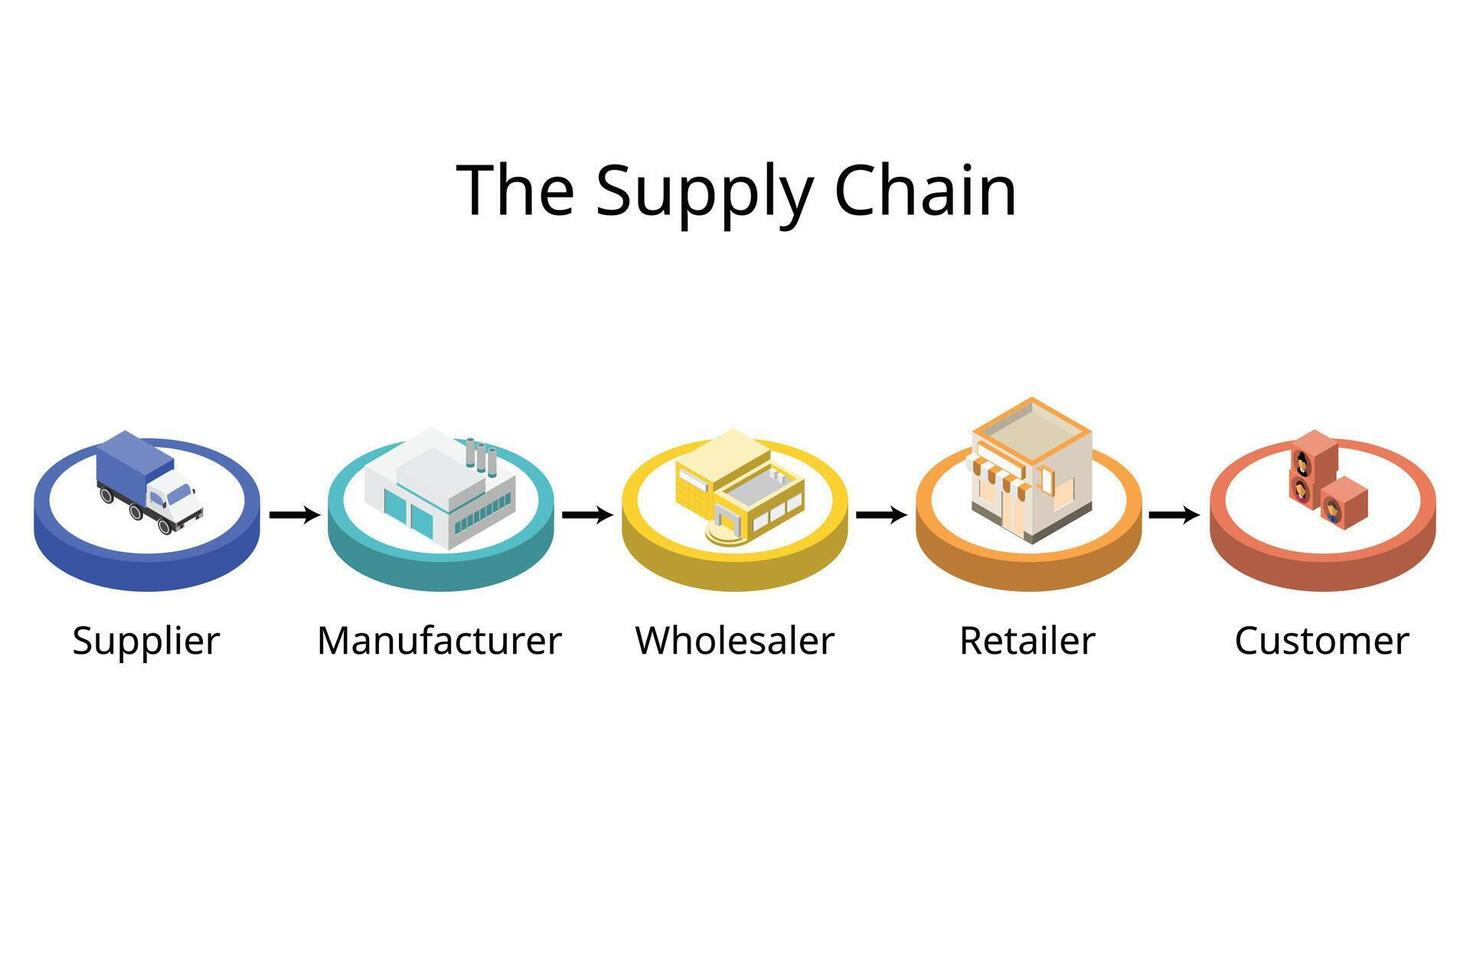
\includegraphics[width=0.7\textwidth]{supply_chain_flow.png} % replace
   \caption{Supply chain flow diagram}
   \label{fig:sc-flow}
\end{figure}

\needspace{6\baselineskip}
\section{Why supply chain management and analytics matter}
\nopagebreak[4]
Managing a supply chain directly affects \textbf{profitability, customer trust, and business survival}.
\begin{itemize}[noitemsep, topsep=0pt]
   \item \textbf{Profitability:} A well‑managed supply chain reduces unnecessary costs (excess inventory, long storage, inefficient transport). These savings go directly to the bottom line.
   \item \textbf{Customer trust:} When a product is available and arrives on time, customers come back. When it doesn't, they switch to competitors – often forever.
   \item \textbf{Business resilience:} A single disruption (port strike, natural disaster, pandemic) can halt production for weeks. Good supply chain design helps avoid or quickly recover from such shocks.
\end{itemize}

\begin{tcolorbox}[colback=lightbg, colframe=gold, boxrule=1pt, arc=4pt, left=6pt, right=6pt, top=6pt, bottom=6pt, fonttitle=\bfseries\color{navy}, title=Research evidence]
\textbf{Research evidence:}  
According to a McKinsey study, companies with high‑performing supply chains achieve 15–20\% lower costs and 30–50\% less inventory than average performers.  
Gartner reports that 83\% of supply chain professionals believe analytics will become a core competency within three years.
\end{tcolorbox}

\section{Project context}
This project applies the importance of supply chain analytics by building an \textbf{end‑to‑end data pipeline} – from raw data to visualisation – using modern Big Data technologies.

\textbf{Why this dataset?}  
We chose the \textbf{DataCo SMART SUPPLY CHAIN} dataset (Kaggle) because it simulates a real‑world e‑commerce supply chain and contains realistic anomalies (missing values, duplicates, constant columns) that require cleaning and normalisation. It also spans several years, allowing us to build a time‑series forecasting model.

\section{Dataset presentation}
\begin{itemize}[noitemsep, topsep=0pt]
   \item \texttt{DataCoSupplyChainDataset.csv} – main structured file (~180 000 rows, ~50 columns).
   \item \texttt{DescriptionDataCoSupplyChain.csv} – data dictionary.
   \item \texttt{tokenized\_access\_logs.csv} – unstructured clickstream logs (not used).
\end{itemize}

\section{Project objectives}
The objective is to implement the following pipeline, whose scheme is shown below:

\begin{figure}[H]
   \centering
   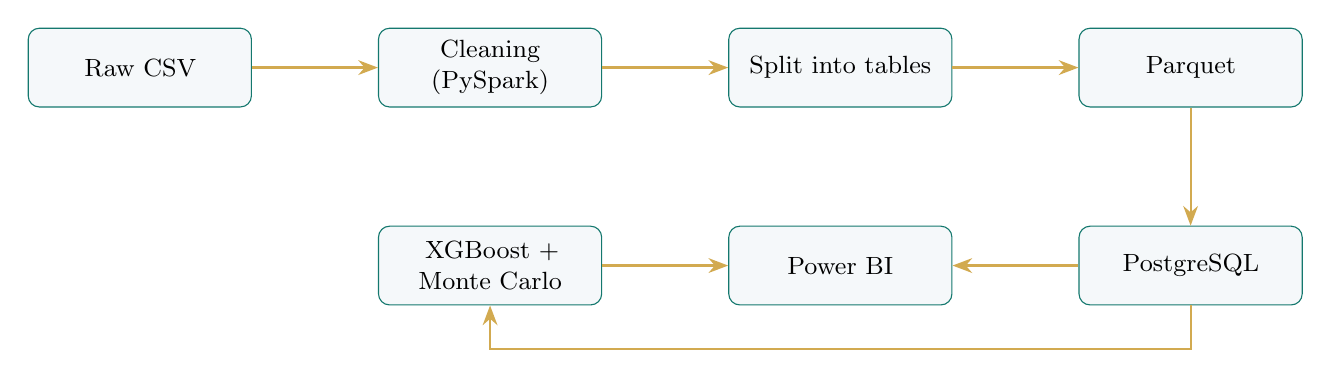
\begin{tikzpicture}[
      block/.style={rectangle, draw=teal, fill=lightbg, text width=2.6cm, align=center, rounded corners, minimum height=1cm, font=\small},
      arrow/.style={->, thick, draw=gold, -{Stealth[length=2.5mm]}}
   ]
      % Row 1 (left to right)
      \node (raw)     [block] at (0,0)              {Raw CSV};
      \node (clean)   [block, right=1.6cm of raw]   {Cleaning (PySpark)};
      \node (split)   [block, right=1.6cm of clean] {Split into tables};
      \node (parquet) [block, right=1.6cm of split] {Parquet};

      % Row 2 (below, right-aligned under Parquet)
      \node (pg)  [block, below=1.5cm of parquet]  {PostgreSQL};
      \node (pbi) [block, left=1.6cm of pg]         {Power BI};
      \node (ml)  [block, left=1.6cm of pbi]        {XGBoost + Monte Carlo};

      % Row 1 arrows
      \draw[arrow] (raw)     -- (clean);
      \draw[arrow] (clean)   -- (split);
      \draw[arrow] (split)   -- (parquet);

      % Vertical connector
      \draw[arrow] (parquet) -- (pg);

      % Row 2: PostgreSQL and ML both feed Power BI
      \draw[arrow] (pg)  -- (pbi);
      \draw[arrow] (ml)  -- (pbi);

      % PostgreSQL also feeds ML – routed below row 2 to avoid crossing Power BI
      \draw[arrow] (pg.south) -- ++(0,-0.55) -| (ml.south);
   \end{tikzpicture}
   \caption{Pipeline architecture}
   \label{fig:pipeline}
\end{figure}

\chapter{Supply Chain Before and After Big Data}
\section{Comparative Table}
\begin{table}[H]
   \centering
   \renewcommand{\arraystretch}{1.3}
   \altrows
   \small
   \caption{Traditional vs Big Data supply chain}
   \label{tab:comparison}
   \begin{tabular}{@{}p{3.2cm}p{4.5cm}p{4.5cm}@{}}
      \toprule
      \textbf{Aspect} & \textbf{Traditional SCM} & \textbf{Big Data‑driven SCM} \\
      \midrule
      Data sources & Limited to internal structured data (ERP, historical sales). & Diverse real‑time sources: IoT, social media, weather, market data. \\
      Forecasting & Static models based on historical averages; higher error rates. & Predictive ML models with real‑time variables; 20–30\% higher accuracy. \\
      Decision‑making & Reactive, intuition‑based, periodic reviews. & Proactive, data‑driven, real‑time insights. \\
      Visibility & Fragmented, siloed, limited end‑to‑end view. & Full transparency via real‑time tracking and digital twins. \\
      Inventory management & Manual, fixed reorder points; overstock/stockouts common. & Real‑time optimisation; 30–50\% cost reduction reported. \\
      Risk management & Reactive crisis management after disruption. & Predictive identification of vulnerabilities and early warnings. \\
      Operational agility & Slow, manual adjustments; rigid plans. & Highly agile, near‑instantaneous response to market changes. \\
      Key technologies & Excel, basic ERP, relational databases. & Hadoop, Spark, IoT, AI/ML, cloud analytics. \\
      \bottomrule
   \end{tabular}
\end{table}
\subsection*{Sources}
{\small\raggedright
\begin{itemize}[noitemsep, topsep=0pt]
   \item Caliber Global. (2025). \textit{How Big Data and Analytics Are Transforming Supply Chain Management}. \url{https://caliber.global/blog/big-data-analytics-supply-chain-management}
   \item Gunasekaran, A. et al. (2025). \textit{A comparative analysis of traditional vs AI‑enabled processes}. World Journal of Advanced Research and Reviews, 15(01), 1762–1769.
   \item Leadafi. (2024). \textit{The Evolution of Supply Chain Management: From Traditional to Digital}. \url{https://leadafi.com/...}
   \item Agidi, R. Y. S. et al. (2024). \textit{An evaluation of current technology in supply chain management}. International Journal of Science and Research Archive, 12(01), 478–491.
   \item Kommula, H. M. (2025). \textit{The role of predictive analytics in enhancing supply chain resilience}. World Journal of Advanced Engineering Technology and Sciences, 15(01), 1762–1769.
   \item Lin, Z. (2024). \textit{Big Data Analytics in Supply Chain Optimization and Risk Management: A case study of Amazon}. SHS Web of Conferences.
\end{itemize}
}

\chapter{Technology Stack and Justification}
\subsection*{\faPython\ PySpark}
We use PySpark for distributed data cleaning and transformation. It handles the 180k‑row dataset efficiently and scales horizontally. PySpark implements the \textbf{MapReduce} paradigm (lazy evaluation, data locality) and is part of the Hadoop ecosystem. This directly addresses the \textbf{Volume} and \textbf{Velocity} challenges of Big Data.

\subsection*{\faDatabase\ PostgreSQL}
PostgreSQL stores our normalised tables (3NF). It enforces primary/foreign keys, supports complex queries, and connects easily to Power BI. It represents the \textbf{structured data} side of the \textbf{Variety} challenge, showing that traditional RDBMS remain essential for clean, transactional data.

\subsection*{\faChartLine\ Power BI}
Power BI creates interactive dashboards for sales, logistics, and forecasts. It connects directly to PostgreSQL and turns raw data into actionable insights. This addresses the \textbf{Value} and \textbf{Veracity} dimensions of Big Data, transforming numbers into business decisions.

\subsection*{\faRobot\ XGBoost}
XGBoost is a gradient boosting algorithm used for demand forecasting. It handles non‑linear relationships and missing values, and provides feature importance. It implements \textbf{predictive analytics} and is a core machine learning tool for generating future insights from historical data.

\subsection*{\faRandom\ Monte Carlo Simulation}
Monte Carlo simulates thousands of demand scenarios to quantify stockout risk. It computes probabilities and safety stock recommendations. This addresses the \textbf{Veracity} (uncertainty) and \textbf{Value} dimensions, turning a point forecast into a risk‑aware decision.

\subsection*{\faGithub\ Git / GitHub}
We use Git for version control with branches (`main`, `dev`, `sprint‑*`, `task/*`), pull requests, and code reviews. While not a Big Data tool, Git ensures \textbf{collaboration} and \textbf{reproducibility}, aligning with professional data engineering practices.

% \section{Summary Table}   <-- REMOVED (title deleted)
\begin{table}[H]
   \centering
   \renewcommand{\arraystretch}{1.3}
   \altrows
   \small
   \caption{Technology stack summary}
   \label{tab:techstack}
   \begin{tabular}{@{}lll@{}}
      \toprule
      Tool & Role & Course link \\
      \midrule
      PySpark & Distributed cleaning, transformation & MapReduce, Hadoop ecosystem, Volume \& Velocity \\
      PostgreSQL & Relational storage, 3NF schema & Structured data (Variety), ACID \\
      Power BI & Interactive dashboards, KPIs & Value \& Veracity, BI, visualisation \\
      XGBoost & Demand forecasting & Predictive analytics, ML, feature importance \\
      Monte Carlo & Risk simulation, stockout probability & Veracity (uncertainty), probabilistic modelling \\
      Git/GitHub & Version control, branch workflow & Collaboration, reproducibility \\
      \bottomrule
   \end{tabular}
\end{table}

\chapter{Project Environment and Architecture}

\section{Operating System and Hardware}
\begin{itemize}[noitemsep, topsep=0pt]
   \item \textbf{Operating System:} Windows 11 (64-bit)
   \item \textbf{Hardware:} Laptop with 16 GB RAM, SSD (all processing local, no cluster)
   \item \textbf{IDE:} Visual Studio Code
\end{itemize}

\section{Folder Structure}
\begin{tcolorbox}[colback=lightbg, colframe=teal, boxrule=1pt, arc=4pt, left=6pt, right=6pt, top=6pt, bottom=6pt, fontupper=\small]
\begin{verbatim}
Supply-Chain-Analysis/
├── data/
│   ├── raw/               # original Kaggle CSV files (ignored by Git)
│   └── staging/           # intermediate Parquet files (cleaned, split, features)
├── notebooks/
│   └── eda.ipynb          # EDA notebook
├── src/                   # Python/PySpark scripts
│   ├── cleaning.py
│   ├── split_tables.py
│   ├── load_postgres.py
│   ├── feature_engineering.py
│   └── xgb_montecarlo.py
├── sql/                   # SQL scripts
│   ├── schema.sql
│   ├── validation.sql
│   └── indexes.sql
├── docs/                  # ERD, UML, report sections
├── powerbi/
│   └── supply_chain.pbix  # Power BI dashboard file
├── models/                # saved XGBoost model (xgboost_demand_model.pkl)
├── reports/               # final report and presentation
├── .gitignore
├── .env.example
├── requirements.txt
├── README.md
└── CONTRIBUTING.md
\end{verbatim}
\end{tcolorbox}

\chapter{How to Run the Project}
\section{Step‑by‑step instructions}
\subsection{Prerequisites}
Python 3.11+, Java 11, PostgreSQL 16, Git, Power BI Desktop (optional).

\subsection{Clone the repository}
\begin{codebox}
git clone https://github.com/onsaissa4/Supply-Chain-Analysis.git
cd Supply-Chain-Analysis
\end{codebox}

\subsection{Create a virtual environment (recommended)}
\begin{codebox}
python -m venv venv
.\venv\Scripts\activate   # Windows
# source venv/bin/activate   # Linux/macOS
\end{codebox}

\subsection{Install Python dependencies}
\begin{codebox}
pip install -r requirements.txt
\end{codebox}
If missing, install manually:
\begin{codebox}
pip install pandas pyspark numpy matplotlib seaborn jupyter psycopg2-binary sqlalchemy scikit-learn xgboost joblib pyarrow python-dotenv
\end{codebox}

\subsection{Download the dataset}
Place the three CSV files from Kaggle into \texttt{data/raw/}.
{\small\raggedright
\url{https://www.kaggle.com/datasets/shashwatwork/dataco-smart-supply-chain-for-big-data-analysis}
\par}

\subsection{PostgreSQL setup}
Start PostgreSQL, create a database \texttt{supply\_chain}:
\begin{codebox}
CREATE DATABASE supply\_chain;
\end{codebox}
Update passwords in \texttt{load\_postgres.py} and \texttt{xgb\_montecarlo.py} if needed.

\subsection{Clean and split the raw data}
\begin{codebox}
python src/cleaning.py
python src/split\_tables.py
\end{codebox}

\subsection{Load data into PostgreSQL}
First run the schema:
\begin{codebox}
psql -U postgres -d supply\_chain -f sql/schema.sql
\end{codebox}
Then load:
\begin{codebox}
python src/load\_postgres.py
\end{codebox}

\subsection{Feature engineering (for ML)}
\begin{codebox}
python src/feature\_engineering.py
\end{codebox}

\subsection{XGBoost training and Monte Carlo simulation}
\begin{codebox}
python src/xgb\_montecarlo.py
\end{codebox}

\subsection{Power BI dashboard}
Open \texttt{powerbi/supply\_chain.pbix} in Power BI Desktop, refresh data.

\subsection{Optional: verify forecast table}
\begin{codebox}
SELECT * FROM demand\_forecast LIMIT 10;
\end{codebox}

\section{Execution time}
Measured on a typical laptop (16 GB RAM, SSD) using PowerShell's \texttt{Measure-Command}.

\begin{table}[H]
   \centering
   \renewcommand{\arraystretch}{1.3}
   \altrows
   \small
   \caption{Execution times of main scripts}
   \label{tab:times}
   \begin{tabular}{@{}lr@{}}
      \toprule
      Script & Time (seconds) \\
      \midrule
      \texttt{cleaning.py} & 31.33 \\
      \texttt{split\_tables.py} & 0.96 \\
      \texttt{load\_postgres.py} & 34.66 \\
      \texttt{feature\_engineering.py} & 19.79 \\
      \texttt{xgb\_montecarlo.py} & 12.08 \\
      \bottomrule
   \end{tabular}
\end{table}

\chapter{UML Diagrams (System Design)}

The UML diagrams below (Class, Use Case, Sequence) provide a visual overview of the system. Their detailed justification is integrated into the relevant sprint descriptions throughout this report.

\section{Class Diagram}
\begin{figure}[H]
   \centering
   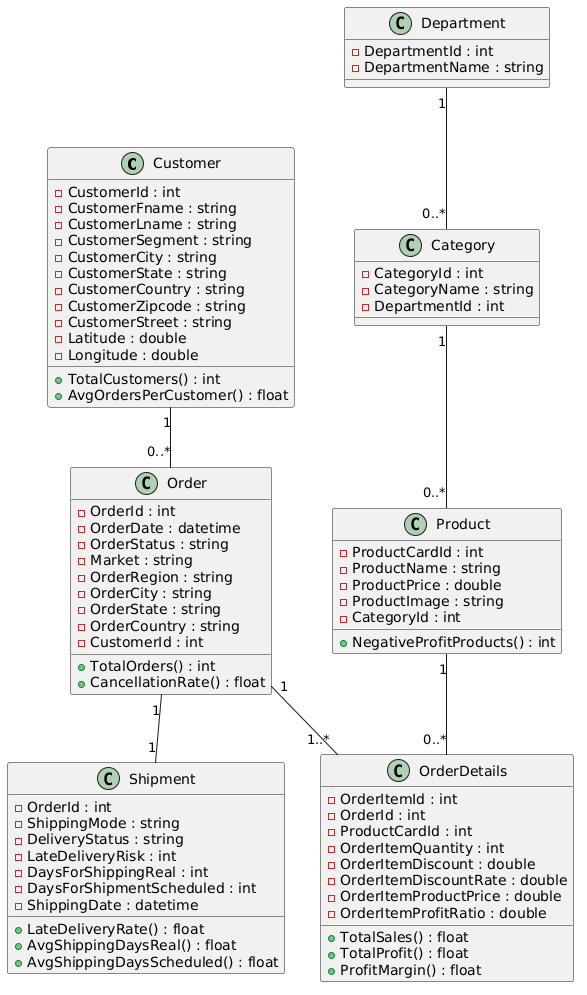
\includegraphics[width=0.8\textwidth, keepaspectratio]{class_diagram.png}
   \caption{Class diagram}
   \label{fig:class}
\end{figure}

\section{Use Case Diagram}
\begin{figure}[H]
   \centering
   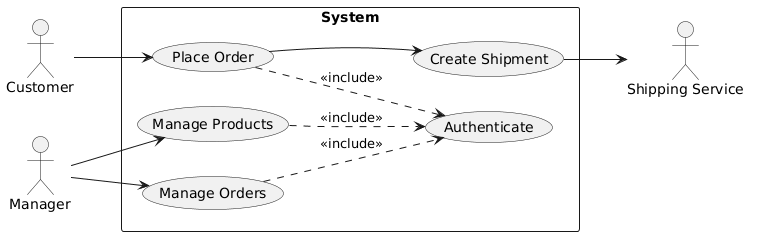
\includegraphics[width=0.8\textwidth]{usecase_diagram.png}
   \caption{Use case diagram}
   \label{fig:usecase}
\end{figure}

\section{Sequence Diagram}
\begin{figure}[H]
   \centering
   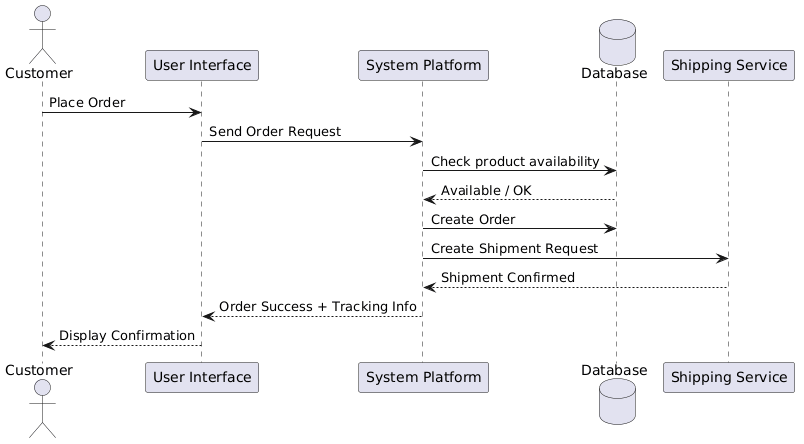
\includegraphics[width=\textwidth]{sequence_diagram.png}
   \caption{Sequence diagram}
   \label{fig:sequence}
\end{figure}

\chapter{Git Workflow Used}
We followed the branching strategy and workflow defined in \texttt{CONTRIBUTING.md}.

\section{Branches}
\begin{itemize}[noitemsep, topsep=0pt]
   \item \textbf{main} – final code (only at the end of the project).
   \item \textbf{dev} – integration branch. Each sprint is merged here after completion.
   \item \textbf{sprint-1} … \textbf{sprint-6} – branches for each sprint.
   \item \textbf{task/*} – temporary branches for individual tasks (e.g., \texttt{task/ons-pandas-eda}).
\end{itemize}

\section{Workflow}
\begin{enumerate}[noitemsep, topsep=0pt]
   \item Always start from the current sprint branch (e.g., \texttt{sprint-1}).
   \item Create a \texttt{task/} branch (e.g., \texttt{task/ons-pandas-eda}).
   \item Work on that branch, commit, and push.
   \item Open a Pull Request (PR) towards the sprint branch.
   \item The other team member reviews and merges.
   \item Once the sprint is finished, merge the sprint branch into \texttt{dev}.
\end{enumerate}

\section{Pull Request Process}
\begin{itemize}[noitemsep, topsep=0pt]
   \item Every PR must be reviewed by the other team member.
   \item After approval, the reviewer merges the PR (or the author merges if the reviewer has no write permissions).
\end{itemize}

\chapter{Sprint Overview (Roadmap)}
\section{7 sprints overview}
\subsection*{Sprint 1 – Environment Setup, EDA, and ERD}
\textbf{Objective:} Set up environment, perform EDA (9‑point checklist), conceive ERD, define cleaning decisions. \\
\textbf{Task repartition:}
\begin{itemize}[noitemsep, topsep=0pt]
   \item Both: environment setup, EDA (shared checklist).
   \item Ons: ERD design.
\end{itemize}

\subsection*{Sprint 2 – Data Cleaning and Splitting (PySpark)}
\textbf{Objective:} Execute cleaning decisions, normalise CSV into seven tables, save Parquet. \\
\textbf{Task repartition:}
\begin{itemize}[noitemsep, topsep=0pt]
   \item Ranime: cleaning script (\texttt{cleaning.py}).
   \item Ons: splitting script (\texttt{split\_tables.py}).
\end{itemize}

\subsection*{Sprint 3 – PostgreSQL Storage}
\textbf{Objective:} Create schema, load data, validate integrity, add indexes. \\
\textbf{Task repartition:}
\begin{itemize}[noitemsep, topsep=0pt]
   \item Ons: schema and loading script.
   \item Ranime: validation and indexes.
\end{itemize}

\subsection*{Sprint 4 – Power BI Dashboards}
\textbf{Objective:} Build historical dashboards (sales, logistics, customers, profitability). \\
\textbf{Task repartition:}
\begin{itemize}[noitemsep, topsep=0pt]
   \item Ons: pages 1 \& 2 (Sales Overview, Logistics \& Delays).
   \item Ranime: pages 3 \& 4 (Customers, Product Profitability).
\end{itemize}

\subsection*{Sprint 5 – Demand Forecasting (XGBoost)}
\textbf{Objective:} Feature engineering for time‑series forecasting. \\
\textbf{Task repartition:}
\begin{itemize}[noitemsep, topsep=0pt]
   \item Ons: \texttt{feature\_engineering.py} (creates \texttt{features.parquet}).
\end{itemize}

\subsection*{Sprint 6 – Risk Simulation (Monte Carlo) and Dashboard Integration}
\textbf{Objective:} Train XGBoost, run Monte Carlo, save to PostgreSQL, visualise in Power BI. \\
\textbf{Task repartition:}
\begin{itemize}[noitemsep, topsep=0pt]
   \item Ranime: \texttt{xgb\_montecarlo.py} (training, simulation, \texttt{demand\_forecast} table).
   \item Ons: Power BI integration of forecast table.
\end{itemize}

\subsection*{Sprint 7 – Report, UML Diagrams, and Presentation}
\textbf{Objective:} Final report, UML diagrams, presentation. \\
\textbf{Task repartition:}
\begin{itemize}[noitemsep, topsep=0pt]
   \item Ranime: UML diagrams (Class, Use Case, Sequence).
   \item Both: co‑writing of report and slides.
\end{itemize}

% ==========================
% Placeholder sections (to be completed later)
% ==========================
\chapter{Sprint 1 – EDA \& ERD}

\section{Overview}
The EDA was performed following a 9‑point checklist (see notebook \texttt{eda.ipynb}). We used \textbf{pandas} for descriptive statistics and visualisations, and \textbf{PySpark} for cardinality aggregations. The analysis directly informed cleaning decisions, business understanding, and the relational model.

\section{Key Findings}

\subsection{Findings that Guided Cleaning Decisions}

\begin{figure}[H]
   \centering
   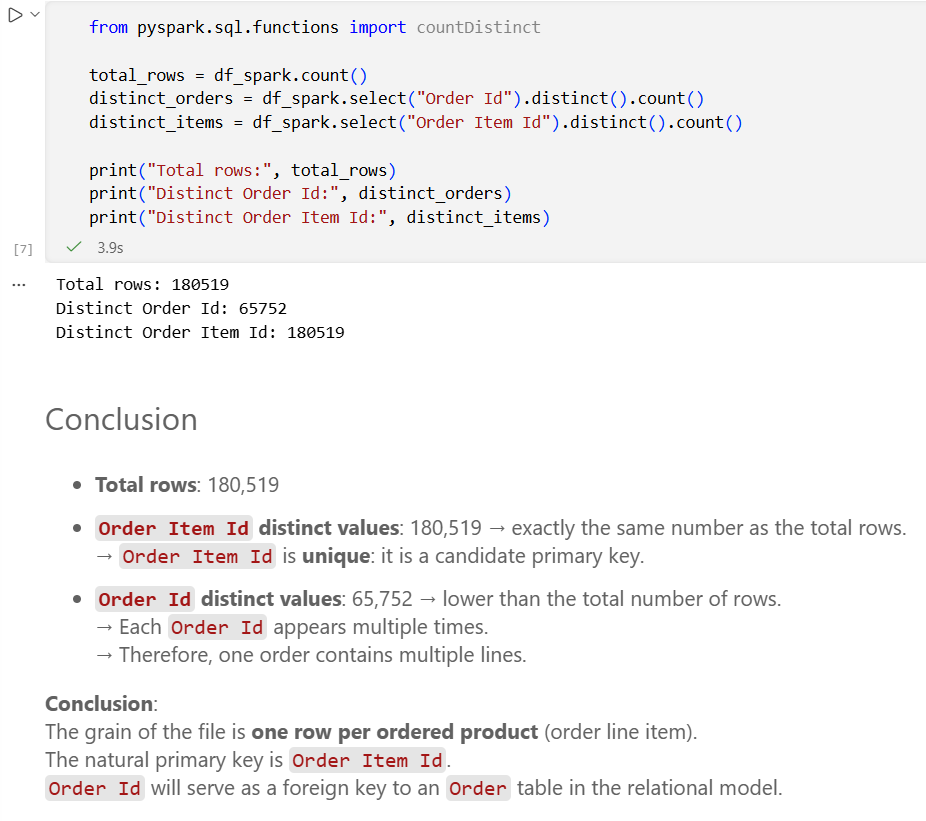
\includegraphics[width=0.8\textwidth]{grain_output.png}
   \caption{Grain analysis: distinct counts of Order Id and Order Item Id.}
   \label{fig:grain}
\end{figure}

\begin{figure}[H]
   \centering
   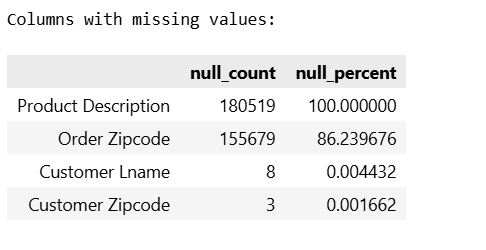
\includegraphics[width=0.8\textwidth]{null_info.png}
   \caption{Columns with missing values.}
   \label{fig:null_info}
\end{figure}

\begin{figure}[H]
   \centering
   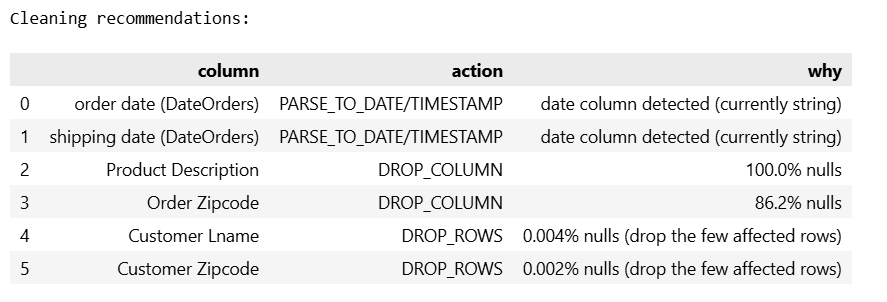
\includegraphics[width=0.8\textwidth]{reco_df.png}
   \caption{Cleaning recommendations (columns to drop, convert, etc.).}
   \label{fig:reco}
\end{figure}

\begin{figure}[H]
   \centering
   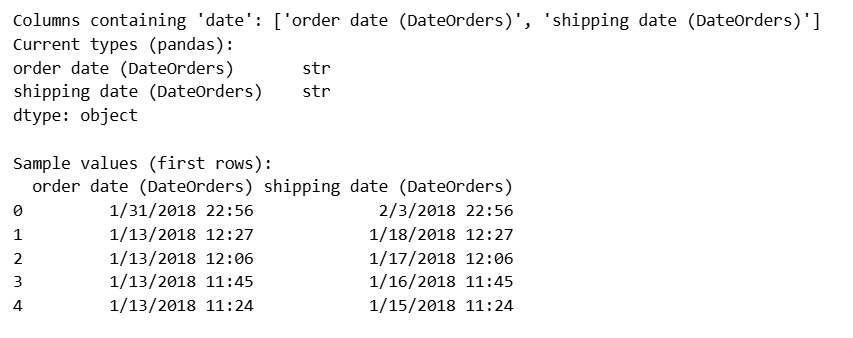
\includegraphics[width=0.8\textwidth]{date_cols.png}
   \caption{Date columns detected as strings.}
   \label{fig:date_cols}
\end{figure}



\subsection{Findings that Supported Business Understanding (EDA Visuals)}
\begin{figure}[H]
   \centering
   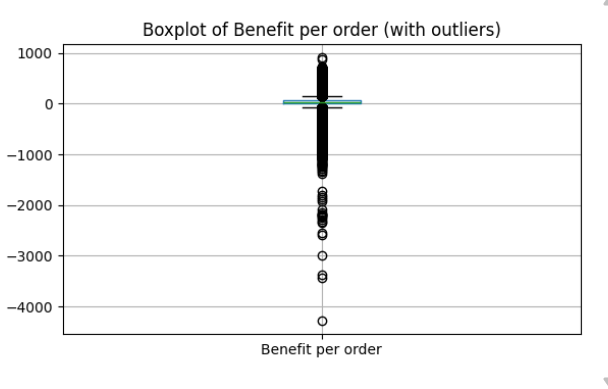
\includegraphics[width=0.8\textwidth]{benefit_boxplot.png}
   \caption{Boxplot of Benefit per order (outliers visible).}
   \label{fig:outlier_box}
\end{figure}

\begin{figure}[H]
   \centering
   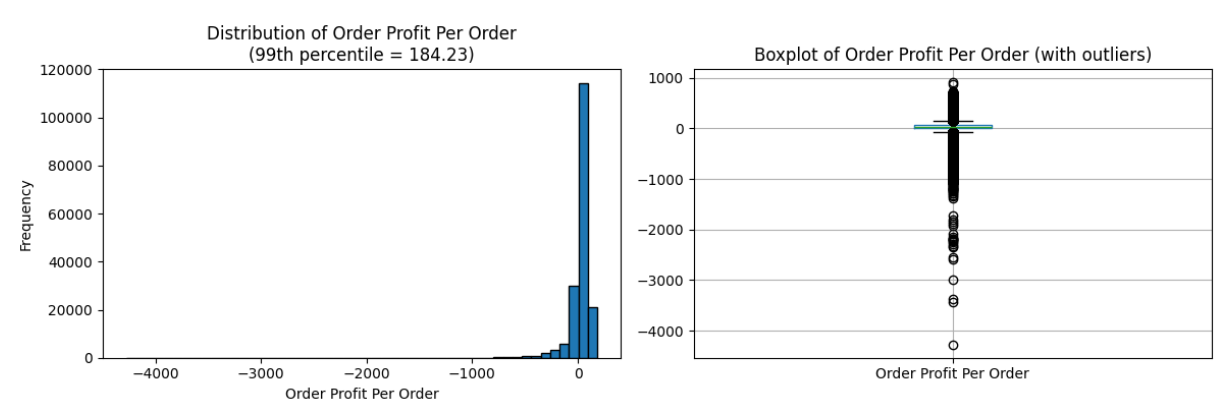
\includegraphics[width=0.9\textwidth]{profit_hist_box.png}
   \caption{Distribution of Benefit per order (histogram and boxplot).}
   \label{fig:profit}
\end{figure}

\begin{figure}[H]
   \centering
   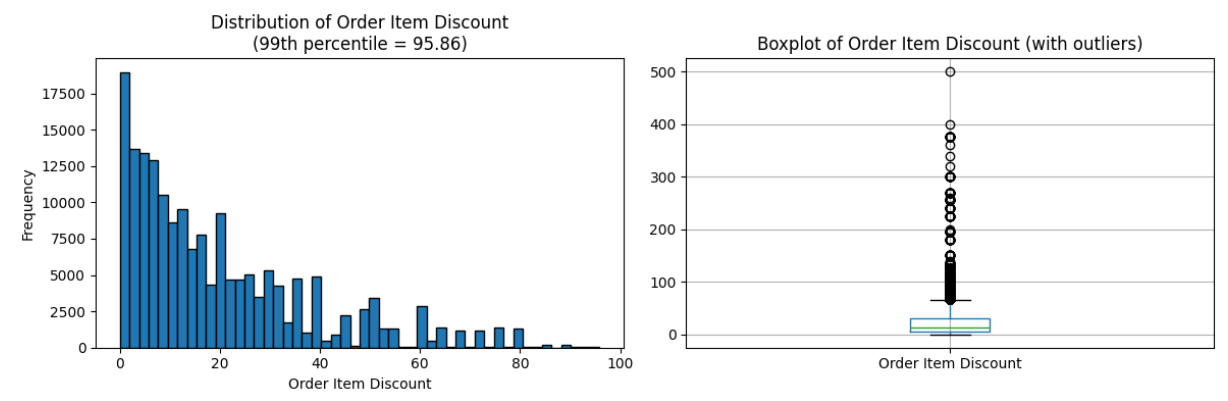
\includegraphics[width=0.9\textwidth]{discount_hist_box.png}
   \caption{Distribution of Order Item Discount.}
   \label{fig:discount}
\end{figure}

\begin{figure}[H]
   \centering
   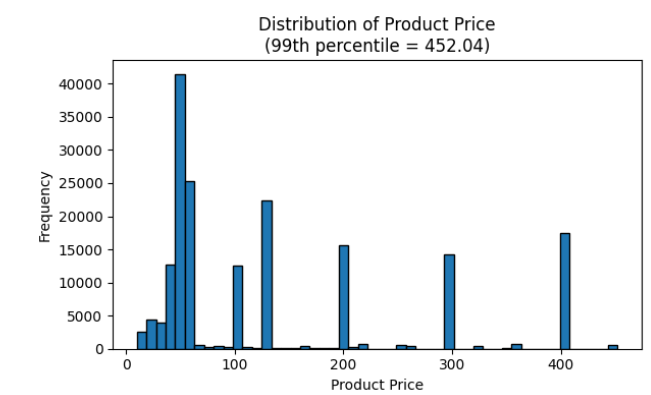
\includegraphics[width=0.8\textwidth]{price_hist.png}
   \caption{Distribution of Product Price (99th percentile).}
   \label{fig:price}
\end{figure}

\begin{figure}[H]
   \centering
   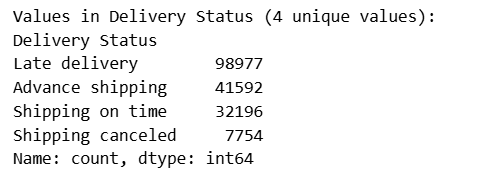
\includegraphics[width=0.7\textwidth]{delivery_status_counts.png}
   \caption{Delivery status frequencies.}
   \label{fig:delivery}
\end{figure}

\begin{figure}[H]
   \centering
   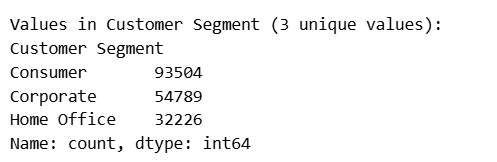
\includegraphics[width=0.7\textwidth]{segment_market_counts.png}
   \caption{Customer segment and market distribution.}
   \label{fig:segment_market}
\end{figure}

\subsection{Findings that Shaped the ERD (Relational Model)}

\begin{figure}[H]
   \centering
   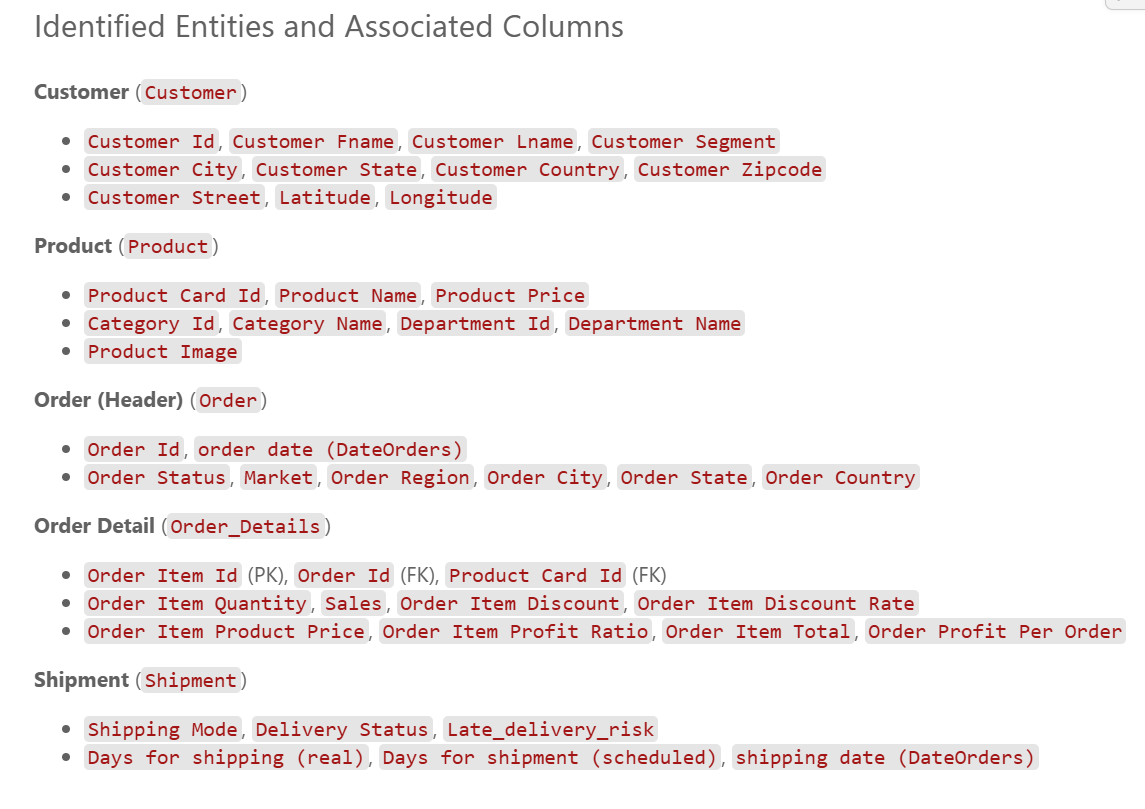
\includegraphics[width=\textwidth]{entity_discovery.png}
   \caption{Entity discovery – column grouping.}
   \label{fig:entity}
\end{figure}

\begin{figure}[H]
   \centering
   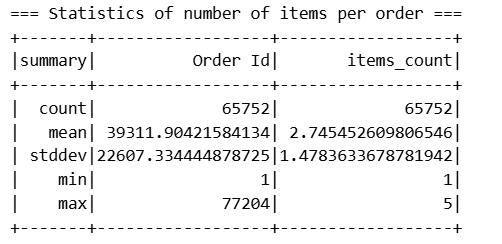
\includegraphics[width=0.8\textwidth]{items_per_order_describe.png}
   \caption{Items per order – statistics.}
   \label{fig:items_per_order}
\end{figure}

\begin{figure}[H]
   \centering
   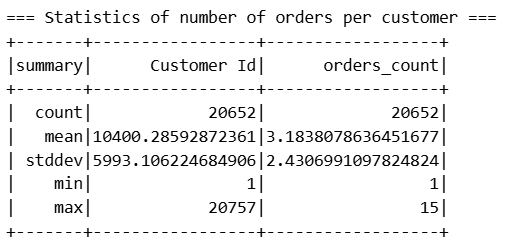
\includegraphics[width=0.8\textwidth]{orders_per_customer_describe.png}
   \caption{Orders per customer – statistics.}
   \label{fig:orders_per_customer}
\end{figure}

\begin{figure}[H]
   \centering
   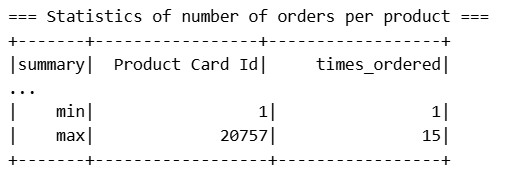
\includegraphics[width=0.8\textwidth]{product_orders_describe.png}
   \caption{Orders per product – statistics.}
   \label{fig:product_orders}
\end{figure}

\begin{figure}[H]
   \centering
   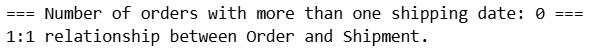
\includegraphics[width=0.8\textwidth]{multi_ship.png}
   \caption{Check for multiple shipments per order (0 orders with >1 shipment).}
   \label{fig:multi_ship}
\end{figure}

\begin{figure}[H]
   \centering
   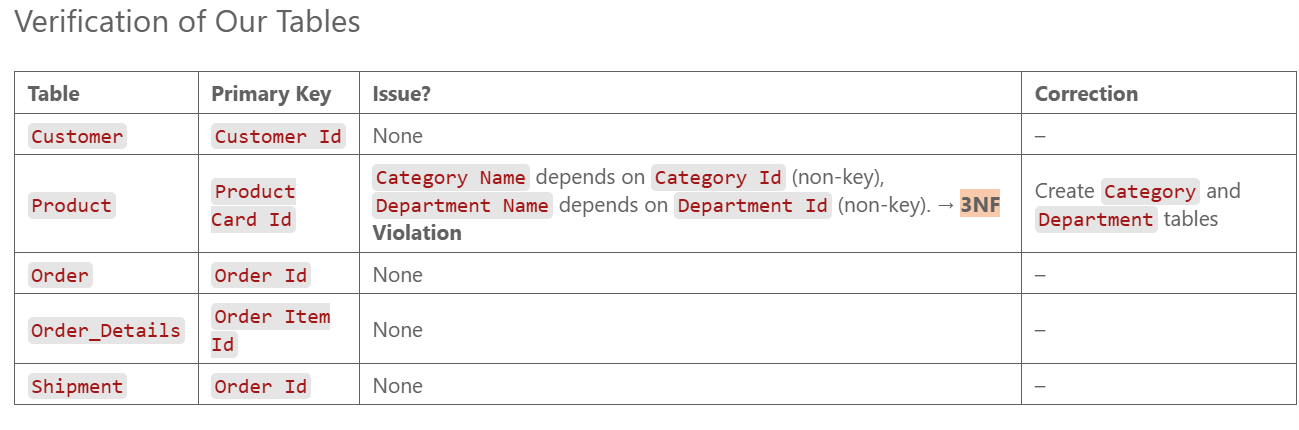
\includegraphics[width=0.8\textwidth]{normalization_table.png}
   \caption{Normalization check – transitive dependencies.}
   \label{fig:normalization}
\end{figure}

\section{ERD Diagram}
\begin{figure}[H]
   \centering
   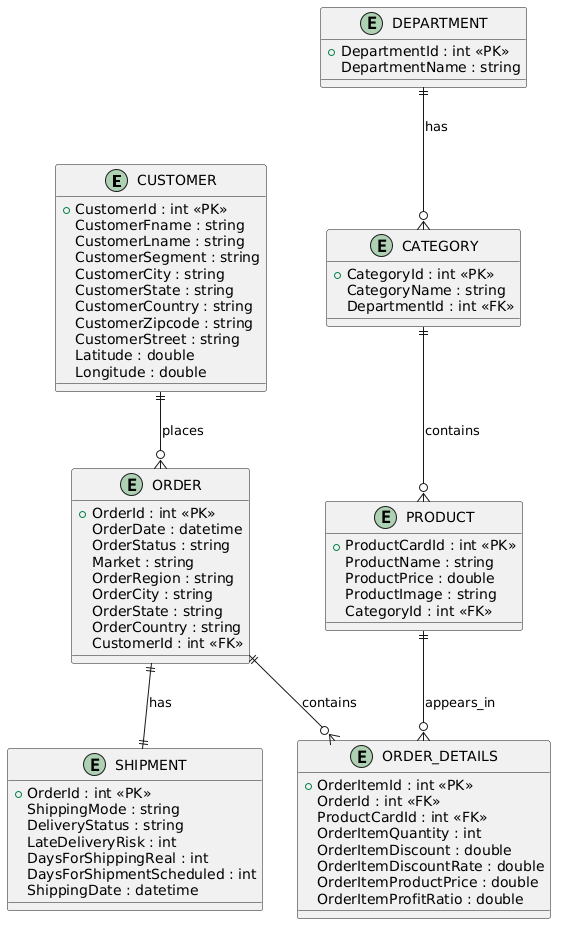
\includegraphics[width=0.8\textwidth]{erd.png}
   \caption{Entity‑Relationship Diagram (3NF) – final model with seven tables.}
   \label{fig:erd}
\end{figure}

\section{Cleaning Decisions Summary}
The table below centralises all cleaning actions (drops, conversions, null handling) that will be implemented in Sprint 2.

\begin{figure}[H]
   \centering
   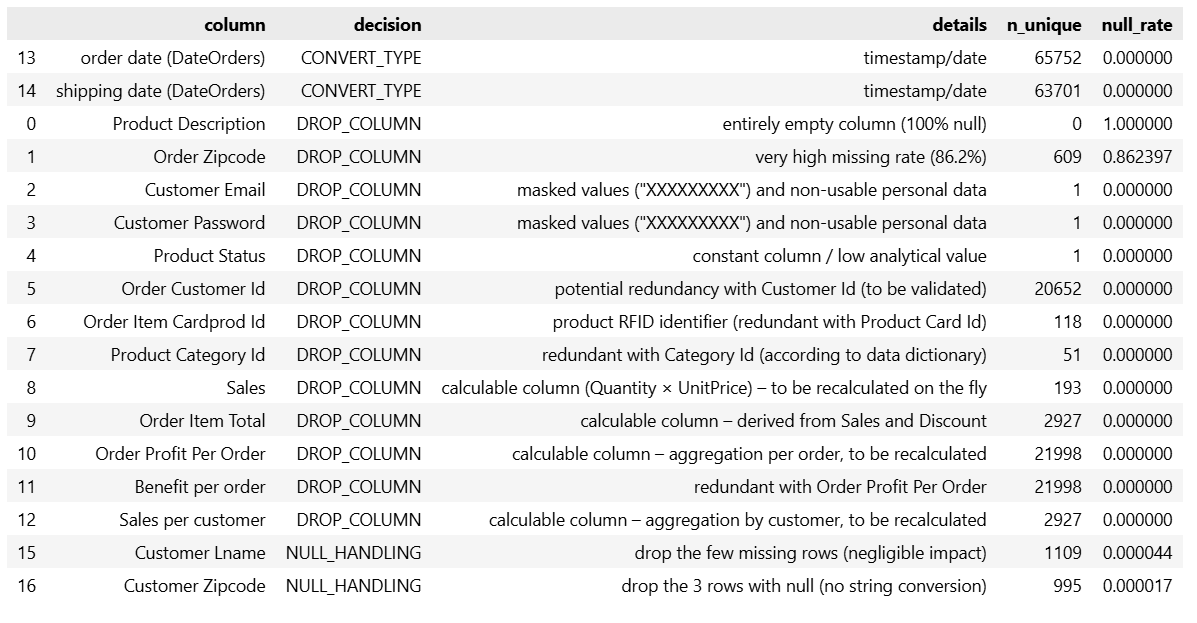
\includegraphics[width=\textwidth]{cleaning_decisions_table.png}
   \caption{Final cleaning decisions table.}
   \label{fig:cleaning_decisions}
\end{figure}

\chapter{Sprint 2 – Data Cleaning and Splitting (PySpark)}

\section{Overview}
The cleaning decisions from Sprint 1 were implemented in PySpark. Two scripts were developed:
\begin{itemize}
   \item \texttt{cleaning.py} (Ranime) – applies column drops, date conversions, and null row removal.
   \item \texttt{split\_tables.py} (Ons) – reads the cleaned Parquet and splits it into seven normalised tables.
\end{itemize}
All intermediate and final data are stored as Parquet files in \texttt{data/staging/}.

\section{Data Cleaning Steps}
\begin{figure}[H]
   \centering
   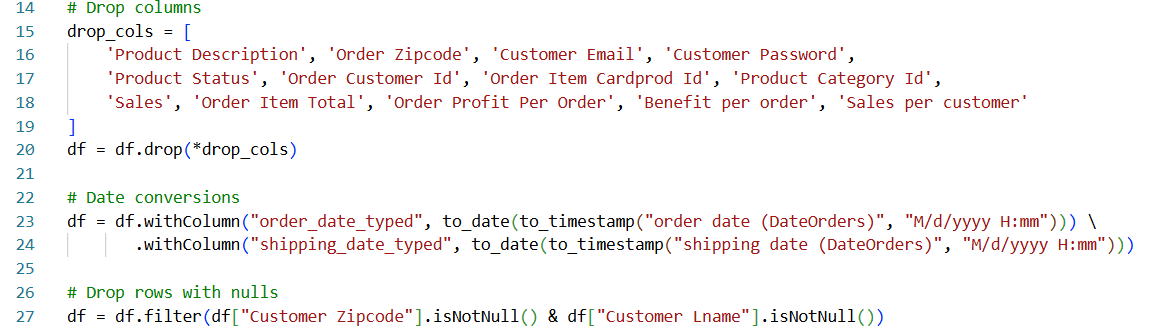
\includegraphics[width=0.8\textwidth]{cleaning_code.png}
   \caption{Key part of \texttt{cleaning.py} (column drops, date conversion, null filtering).}
   \label{fig:cleaning_code}
\end{figure}

\begin{itemize}
   \item Load the raw CSV with PySpark (\texttt{inferSchema=True}).
   \item Drop the columns identified in the cleaning decisions table (Sprint 1, §17).
   \item Convert \texttt{order date (DateOrders)} and \texttt{shipping date (DateOrders)} to \texttt{timestamp} using \texttt{to\_timestamp} and \texttt{to\_date}.
   \item Remove the 8 rows with null in \texttt{Customer Lname} and the 3 rows with null in \texttt{Customer Zipcode}.
   \item Save the cleaned DataFrame as \texttt{cleaned.parquet}.
\end{itemize}

\begin{table}[H]
   \centering
   \caption{Row and column counts before and after cleaning}
   \label{tab:cleaning_counts}
   \begin{tabular}{@{}lcc@{}}
      \toprule
      & \textbf{Before cleaning} & \textbf{After cleaning} \\
      \midrule
      Number of rows & 180 519 & 180 508 \\
      Number of columns & 53 & 42 \\
      \bottomrule
   \end{tabular}
\end{table}

\section{Splitting into Normalised Tables}
\begin{figure}[H]
   \centering
   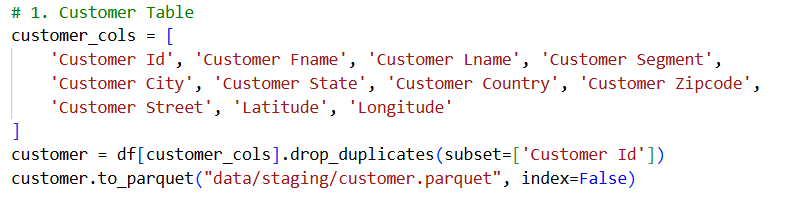
\includegraphics[width=0.8\textwidth]{split_code.png}
   \caption{Key part of \texttt{split\_tables.py} (creating seven DataFrames).}
   \label{fig:split_code}
\end{figure}

Seven separate DataFrames are created by selecting the relevant columns and dropping duplicates on the primary key. The resulting row counts are:

\begin{table}[H]
   \centering
   \caption{Row counts of the split tables}
   \label{tab:split_counts}
   \begin{tabular}{@{}lr@{}}
      \toprule
      Table & Number of rows \\
      \midrule
      \texttt{customer} & 20 652 \\
      \texttt{department} & 11 \\
      \texttt{category} & 50 \\
      \texttt{product} & 118 \\
      \texttt{order} & 65 752 \\
      \texttt{order\_details} & 180 508 \\
      \texttt{shipment} & 65 752 \\
      \bottomrule
   \end{tabular}
\end{table}

Each DataFrame is exported to Parquet in \texttt{data/staging/}.

\begin{figure}[H]
   \centering
   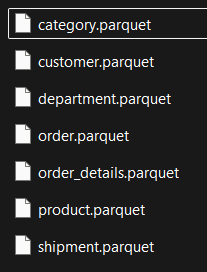
\includegraphics[width=0.8\textwidth]{staging_files.png}
   \caption{List of generated Parquet files in \texttt{data/staging/}.}
   \label{fig:staging_files}
\end{figure}

\section{Result}
After running both scripts, the \texttt{data/staging/} directory contains the seven normalised Parquet files, ready for PostgreSQL loading (Sprint 3).

\chapter{Sprint 3 – PostgreSQL Storage}

\section{Overview}
After generating the seven Parquet files, we loaded them into PostgreSQL. The following scripts were used:
\begin{itemize}
   \item \texttt{sql/schema.sql} – creates the database tables with primary keys, foreign keys, and constraints.
   \item \texttt{src/load\_postgres.py} – reads the Parquet files and inserts data into PostgreSQL.
   \item \texttt{sql/validation.sql} – checks referential integrity and row counts.
   \item \texttt{sql/indexes.sql} – adds performance indexes on foreign keys and date columns.
\end{itemize}

\section{Schema Creation}
\begin{figure}[H]
   \centering
   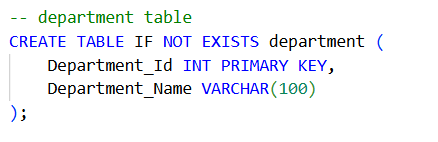
\includegraphics[width=0.8\textwidth]{schema_code.png}
   \caption{Part of \texttt{sql/schema.sql} (example: \texttt{CREATE TABLE department})}
   \label{fig:schema_code}
\end{figure}
The schema defines the seven tables (\texttt{customer}, \texttt{department}, \texttt{category}, \texttt{product}, \texttt{order\_table}, \texttt{order\_details}, \texttt{shipment}) with appropriate data types, primary keys, and foreign keys.

\section{Data Loading}
\begin{figure}[H]
   \centering
   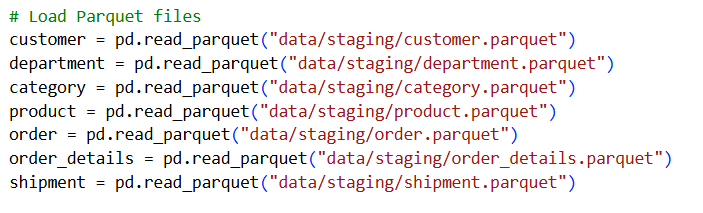
\includegraphics[width=0.8\textwidth]{load_code.png}
   \caption{Key part of \texttt{load\_postgres.py} (connection, truncation, loading)}
   \label{fig:load_code}
\end{figure}
The loading script:
\begin{itemize}
   \item Connects to PostgreSQL using \texttt{sqlalchemy}.
   \item Reads each Parquet file with \texttt{pandas}.
   \item Renames columns (spaces → underscores, lowercasing) to match SQL names.
   \item Truncates tables before loading (to avoid duplicate key errors).
   \item Loads data in the correct order (tables without foreign keys first).
\end{itemize}

\subsection{Row Counts After Loading}
The row counts in PostgreSQL exactly match the Parquet files, confirming successful loading.

\begin{table}[H]
   \centering
   \caption{Row counts of PostgreSQL tables}
   \label{tab:postgres_counts}
   \begin{tabular}{@{}lr@{}}
      \toprule
      Table & Number of rows \\
      \midrule
      \texttt{customer} & 20 652 \\
      \texttt{department} & 11 \\
      \texttt{category} & 50 \\
      \texttt{product} & 118 \\
      \texttt{order\_table} & 65 752 \\
      \texttt{order\_details} & 180 508 \\
      \texttt{shipment} & 65 752 \\
      \bottomrule
   \end{tabular}
\end{table}

\begin{figure}[H]
   \centering
   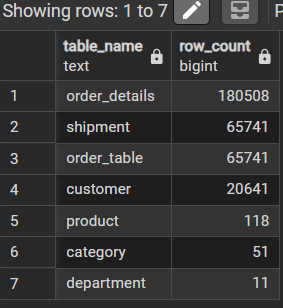
\includegraphics[width=0.8\textwidth]{row_counts_sql.png}
   \caption{Output of \texttt{SELECT COUNT(*) FROM ...} queries}
   \label{fig:row_counts_sql}
\end{figure}

\section{Validation}
\begin{figure}[H]
   \centering
   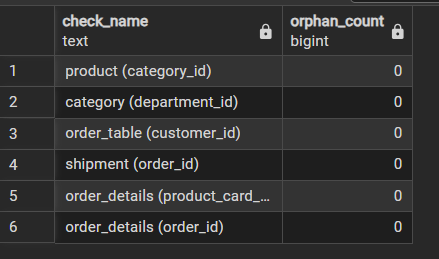
\includegraphics[width=0.8\textwidth]{validation_output.png}
   \caption{Output of validation queries (all zeros indicate no integrity issues)}
   \label{fig:validation_output}
\end{figure}
The \texttt{validation.sql} script checks:
\begin{itemize}
   \item Orphan foreign keys (e.g., \texttt{order\_table.customer\_id} not in \texttt{customer}).
   \item Duplicate primary keys.
   \item Null values in mandatory columns.
\end{itemize}
All checks returned zero, confirming referential integrity.

\section{Indexing}
\begin{figure}[H]
   \centering
   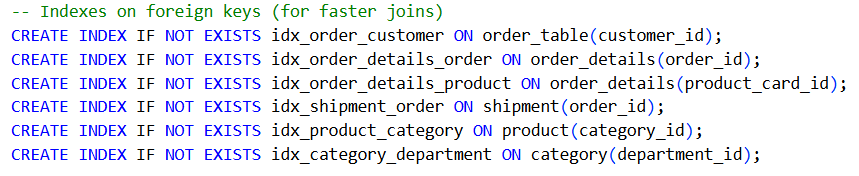
\includegraphics[width=0.8\textwidth]{indexes_code.png}
   \caption{Part of \texttt{sql/indexes.sql} (example: \texttt{CREATE INDEX ...})}
   \label{fig:indexes_code}
\end{figure}
Indexes were added on:
\begin{itemize}
   \item Foreign keys: \texttt{order\_table.customer\_id}, \texttt{order\_details.order\_id}, \\
         \texttt{order\_details.product\_card\_id}, \texttt{shipment.order\_id}.
   \item Frequently searched columns: \texttt{order\_table.order\_date\_typed}, \\
         \texttt{shipment.shipping\_date\_typed}.
\end{itemize}

\section{Result}
After running the scripts, the PostgreSQL database \texttt{supply\_chain} contains the seven fully normalised tables with integrity constraints and indexes, ready for Power BI and machine learning.

\chapter{Sprint 4 – Power BI Dashboards (Historical KPIs)}

\section{Overview}
Power BI Desktop was connected to PostgreSQL (Import mode). Four interactive dashboard pages were created, each answering a specific set of supply chain questions. All visuals are based on the cleaned and normalised tables (no forecast – that is added in Sprint 6).

The following KPIs were defined using DAX measures:

\begin{itemize}
   \item \textbf{Total Sales} = SUM(order\_details[sales])
   \item \textbf{Total Profit} = SUMX(order\_details, order\_details[order\_item\_quantity] * order\_details[order\_item\_product\_price] * order\_details[order\_item\_profit\_ratio])
   \item \textbf{Profit Margin} = [Total Profit] / [Total Sales]
   \item \textbf{Late Delivery Rate} = AVERAGE(shipment[late\_delivery\_risk])
   \item \textbf{Avg Shipping Days Real} = AVERAGE(shipment[days\_for\_shipping\_real])
   \item \textbf{Avg Shipping Days Scheduled} = AVERAGE(shipment[days\_for\_shipment\_scheduled])
   \item \textbf{Total Customers} = DISTINCTCOUNT(order\_table[customer\_id])
   \item \textbf{Total Orders} = COUNTROWS(order\_table)
   \item \textbf{Avg Orders per Customer} = [Total Orders] / [Total Customers]
   \item \textbf{Cancellation Rate} = CALCULATE(COUNTROWS(order\_table), order\_table[order\_status] = "CANCELED") / [Total Orders]
   \item \textbf{Negative Profit Products} = COUNTROWS(FILTER(VALUES(product[product\_name]), [Total Profit] < 0))
\end{itemize}

\section{Page 1 – Sales Overview}
\textbf{KPIs displayed:} Total Sales, Total Profit, Profit Margin.

\begin{itemize}
   \item \textbf{Line chart:} Sales trend over time (axis: \texttt{order\_date\_typed}) – shows seasonality and growth.
   \item \textbf{Bar chart:} Top 10 products by sales – identifies best‑selling items.
   \item \textbf{Donut chart:} Sales by product category – highlights which categories drive revenue.
   \item \textbf{Slicers:} Category and date range for filtering.
\end{itemize}

\textbf{Business justification:} These visuals help the sales manager monitor performance, identify top products, and understand category contributions.

\begin{figure}[H]
   \centering
   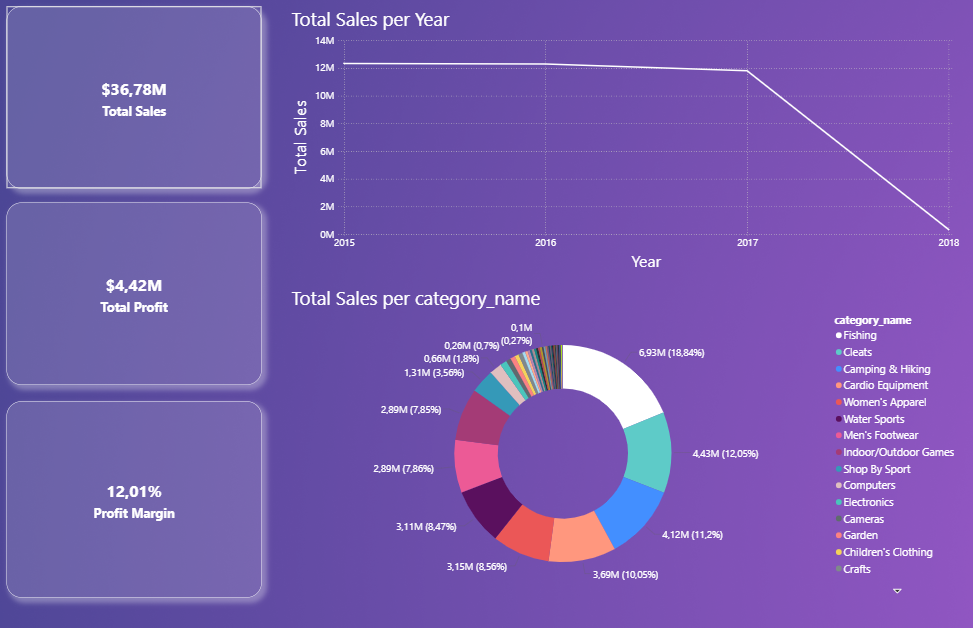
\includegraphics[width=\textwidth]{sales_overview.png}
   \caption{Sales Overview page}
   \label{fig:sales_overview}
\end{figure}

\section{Page 2 – Logistics \& Delays}
\textbf{KPIs displayed:} Late Delivery Rate, Avg Shipping Days Real, Avg Shipping Days Scheduled.

\begin{itemize}
   \item \textbf{Bar chart:} Late delivery rate by shipping mode – shows which carrier is most reliable.
   \item \textbf{Bar chart:} Late delivery rate by order region – identifies geographic areas with delays.
   \item \textbf{Table:} Comparison of real vs scheduled shipping days per shipping mode.
\end{itemize}

\textbf{Business justification:} The logistics manager can assess carrier performance and regional delays, enabling corrective actions.

\begin{figure}[H]
   \centering
   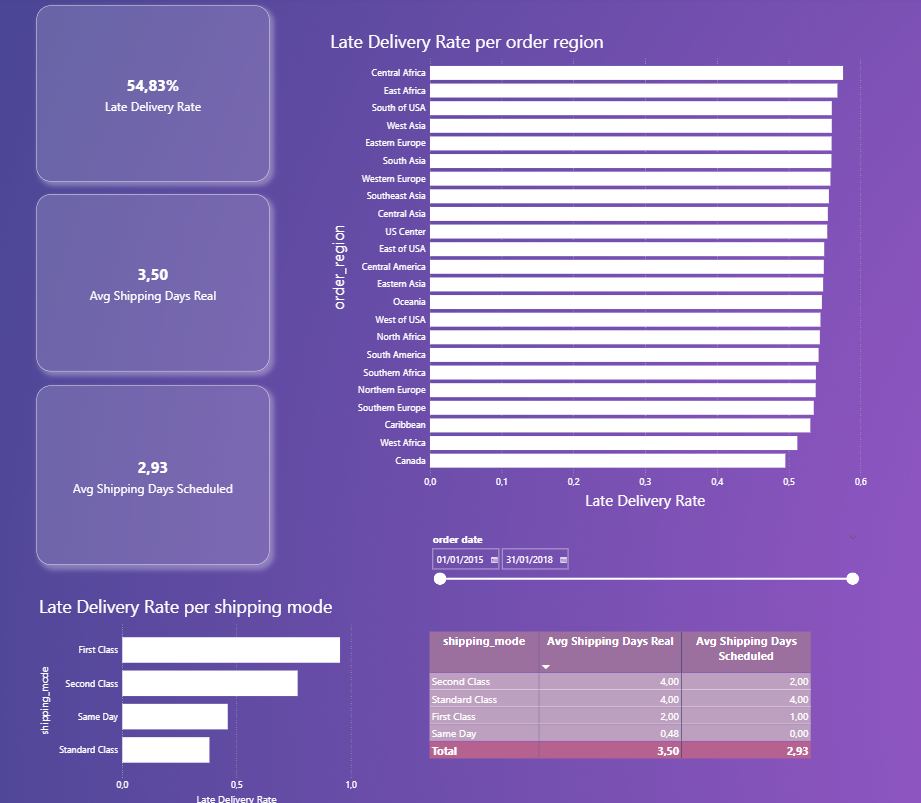
\includegraphics[width=\textwidth]{logistics_page.png}
   \caption{Logistics \& Delays page}
   \label{fig:logistics_page}
\end{figure}

\section{Page 3 – Customers}
\textbf{KPIs displayed:} Total Customers, Avg Orders per Customer.

\begin{itemize}
   \item \textbf{Bar chart:} Sales by customer segment – reveals which segment (Consumer, Corporate, Home Office) contributes most.
   \item \textbf{Table:} Top 10 customers by sales – helps focus retention efforts.
\end{itemize}

\textbf{Business justification:} Marketing and sales teams can tailor campaigns to high‑value segments and loyal customers.

\begin{figure}[H]
   \centering
   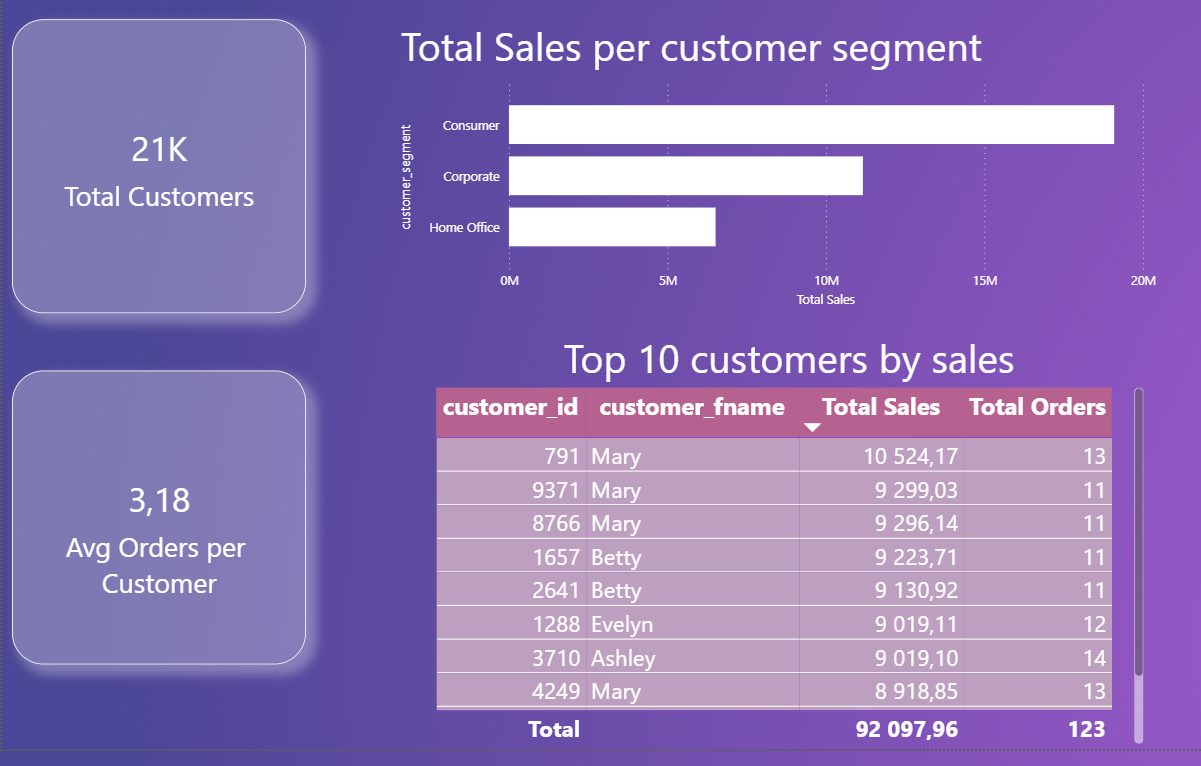
\includegraphics[width=\textwidth]{customers_page.png}
   \caption{Customers page}
   \label{fig:customers_page}
\end{figure}

\section{Page 4 – Product Profitability}
\textbf{KPIs displayed:} Negative Profit Products, Cancellation Rate.

\begin{itemize}
   \item \textbf{Bar chart:} Profit by product (top 10 and bottom 10) – shows most and least profitable items.
   \item \textbf{Scatter plot:} Discount vs profit ratio (coloured by category) – visualises the impact of discounts on profitability.
   \item \textbf{Table:} Products with negative profit – list of loss‑making products.
\end{itemize}

\textbf{Business justification:} The product manager can identify underperforming products, adjust pricing or promotions, and analyse discount effectiveness.

\begin{figure}[H]
   \centering
   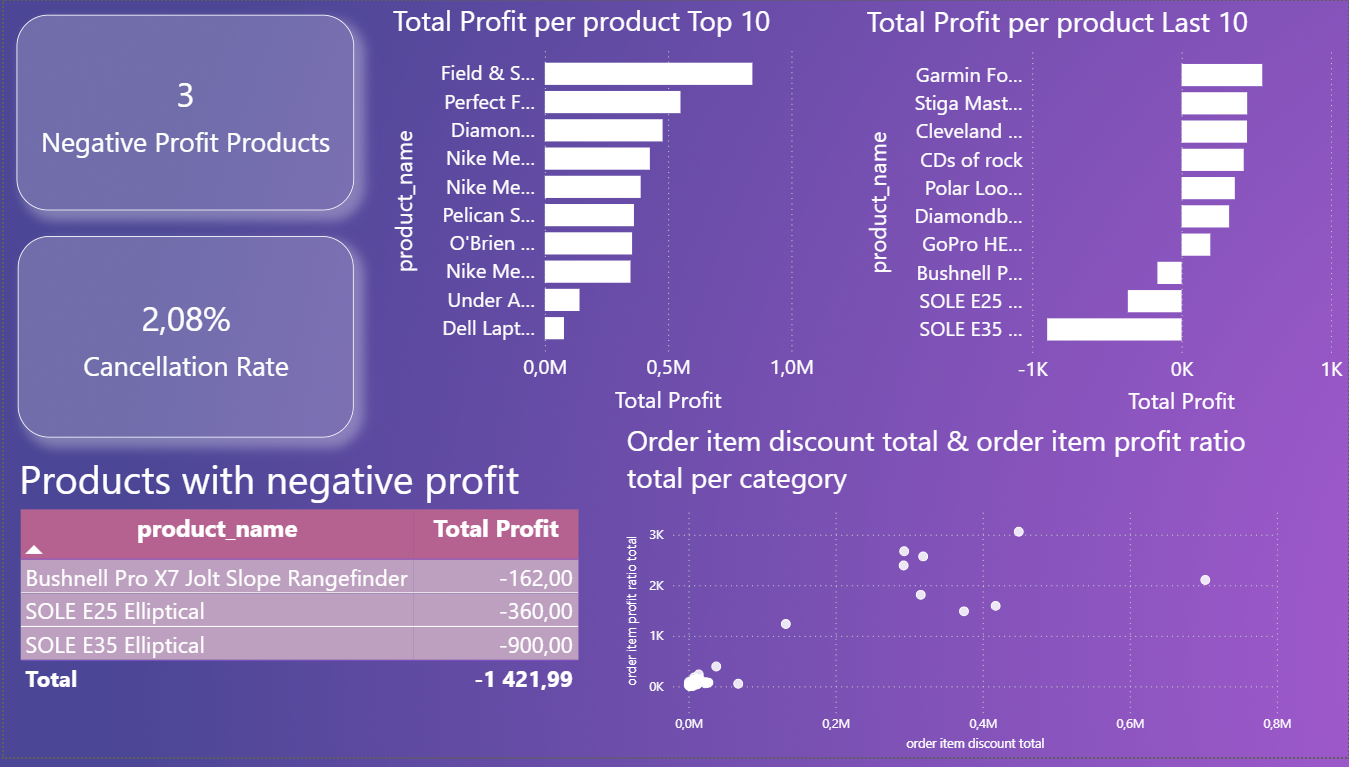
\includegraphics[width=\textwidth]{profitability_page.png}
   \caption{Product Profitability page}
   \label{fig:profitability_page}
\end{figure}

\section{Note on Forecast Integration}
The demand forecast and stockout risk page (using the \texttt{demand\_forecast} table) was added later in Sprint 6 and is described in that chapter. The four pages above cover only historical KPIs.

\chapter{Sprint 5 – Feature Engineering for XGBoost}

\section{Overview}
The goal of this sprint was to prepare a time‑series dataset for demand forecasting. The script \texttt{feature\_engineering.py} (Ons) creates a feature table \texttt{features.parquet} from the cleaned PostgreSQL tables (\texttt{order\_details}, \texttt{order}, \texttt{product}, \texttt{category}). This table is used exclusively by Sprint 6 (XGBoost training and Monte Carlo simulation).

\section{Feature Engineering Steps}
\begin{figure}[H]
   \centering
   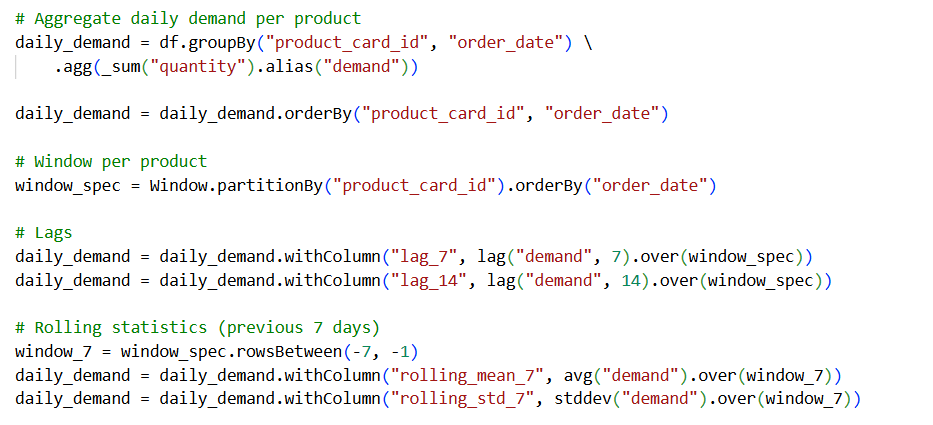
\includegraphics[width=0.8\textwidth]{fe_code.png}
   \caption{Key part of \texttt{feature\_engineering.py} (aggregation, lag creation, target definition).}
   \label{fig:fe_code}
\end{figure}

The following steps were performed:
\begin{enumerate}
   \item Load the cleaned Parquet files (\texttt{order\_details.parquet}, \texttt{order.parquet}, \texttt{product.parquet}, \texttt{category.parquet}).
   \item Aggregate daily demand per product: sum of \texttt{order\_item\_quantity} grouped by \texttt{product\_card\_id} and \texttt{order\_date\_typed}.
   \item Create lag features: \texttt{lag\_7} and \texttt{lag\_14} (demand of the same product 7 and 14 days ago).
   \item Compute rolling statistics: \texttt{rolling\_mean\_7} and \texttt{rolling\_std\_7} over the previous 7 days.
   \item Add calendar features: \texttt{day\_of\_week}, \texttt{month}, \texttt{is\_weekend}.
   \item Join product category (\texttt{category\_name}) from the \texttt{category} table.
   \item Define the target variable: \texttt{demand\_next\_7} = total demand of the next 7 days (sum of future \texttt{demand}).
   \item Drop rows with null values (rows at the beginning or end of the time series).
   \item Save the result as \texttt{features.parquet} in \texttt{data/staging/}.
\end{enumerate}

\section{Output}
The final dataset contains \textbf{20,663 rows} and includes the following columns:

\begin{verbatim}
product_card_id, date, demand, lag_7, lag_14, rolling_mean_7, rolling_std_7,
day_of_week, month, is_weekend, product_category, demand_next_7
\end{verbatim}

\begin{figure}[H]
   \centering
   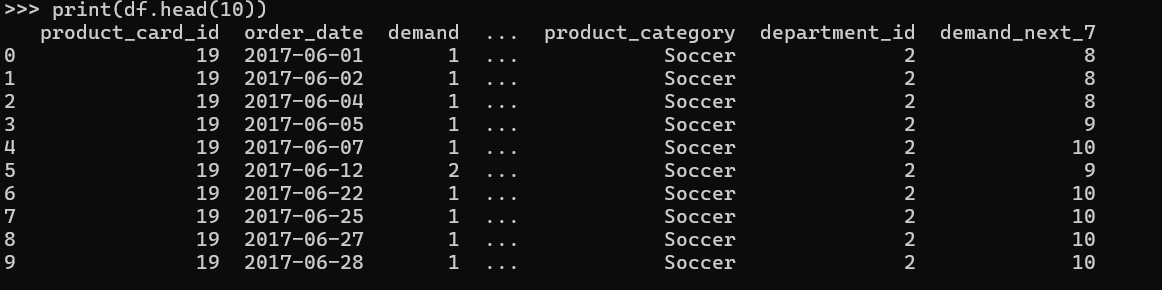
\includegraphics[width=0.8\textwidth]{features_head.png}
   \caption{First few rows of the generated \texttt{features.parquet}.}
   \label{fig:features_head}
\end{figure}

\begin{figure}[H]
   \centering
   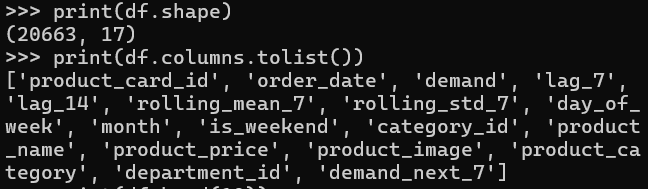
\includegraphics[width=0.8\textwidth]{features_info.png}
   \caption{Summary info of the feature table (shape, columns, data types).}
   \label{fig:features_info}
\end{figure}

\section{Result}
The \texttt{features.parquet} file is now ready for training the XGBoost demand forecasting model (Sprint 6).

\chapter{Sprint 6 – Demand Forecasting, Risk Simulation, and Dashboard Integration}

\section{Overview}
This sprint combines XGBoost training (demand forecasting) and Monte Carlo simulation (stockout risk) into a single script \texttt{xgb\_montecarlo.py} (Ranime). The script uses the feature table \texttt{features.parquet} from Sprint 5. Results are saved to a PostgreSQL table \texttt{demand\_forecast}, which is then integrated into Power BI by Ons.

\section{XGBoost Training and Evaluation}
\begin{figure}[H]
   \centering
   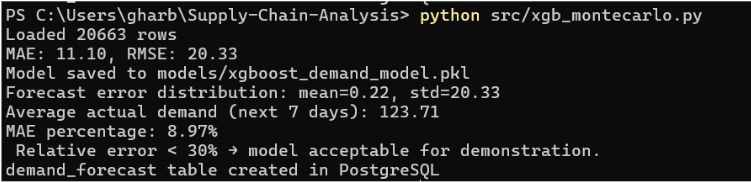
\includegraphics[width=0.8\textwidth]{xgboost_output.png}
   \caption{Output of \texttt{xgb\_montecarlo.py} showing MAE, RMSE, relative error, and model save confirmation.}
   \label{fig:xgboost_output}
\end{figure}

The following steps were performed:
\begin{itemize}
   \item Load \texttt{features.parquet} with pandas.
   \item Features: \texttt{lag\_7}, \texttt{lag\_14}, \texttt{rolling\_mean\_7}, \texttt{rolling\_std\_7}, \texttt{day\_of\_week}, \texttt{month}, \texttt{is\_weekend}, \texttt{product\_category} (one‑hot encoded).
   \item Target: \texttt{demand\_next\_7}.
   \item Train/test split (80/20, random).
   \item XGBoost regressor parameters: \texttt{n\_estimators=100}, \texttt{learning\_rate=0.1}, \texttt{max\_depth=5}.
   \item Evaluation metrics: MAE = 11.10, RMSE = 20.33, relative error = 8.97\% (acceptable <30\%).
   \item Save trained model as \texttt{xgboost\_demand\_model.pkl} in \texttt{models/}.
\end{itemize}

\section{Monte Carlo Simulation for Stockout Risk}
\begin{figure}[H]
   \centering
   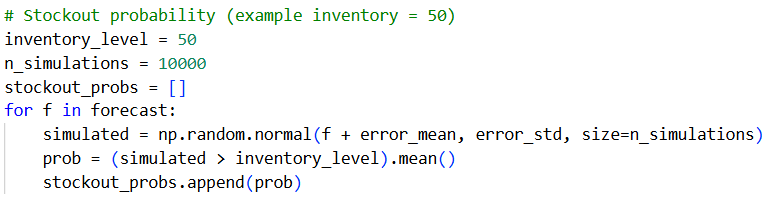
\includegraphics[width=0.8\textwidth]{montecarlo_code.png}
   \caption{Key part of the script showing Monte Carlo simulation loop (error distribution calculation).}
   \label{fig:montecarlo_code}
\end{figure}

\begin{itemize}
   \item Compute forecast errors on the test set: mean error = 0.22, standard deviation = 20.33.
   \item For each row in the full dataset, generate 10 000 simulated demand scenarios using a normal distribution with the forecast as mean and the error standard deviation.
   \item For a given inventory level (example: 50 units), calculate the stockout probability = proportion of simulations where demand > inventory.
   \item This probability is stored per row (later aggregated per product category in Power BI).
\end{itemize}

\section{Saving Results to PostgreSQL – \texttt{demand\_forecast} Table}
\begin{figure}[H]
   \centering
   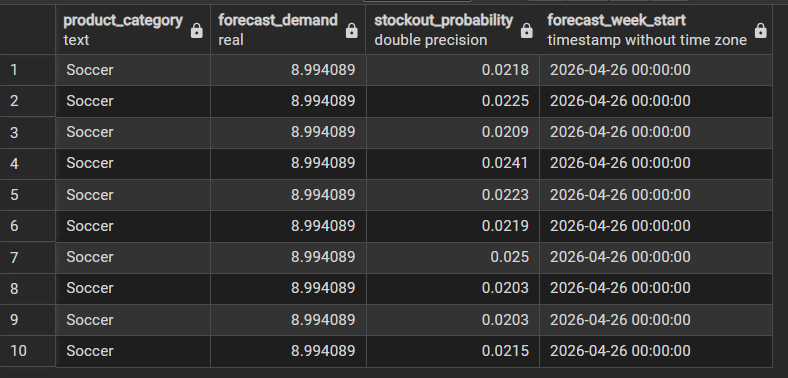
\includegraphics[width=0.8\textwidth]{demand_forecast_table.png}
   \caption{First few rows of the \texttt{demand\_forecast} table in pgAdmin.}
   \label{fig:demand_forecast_table}
\end{figure}

The script creates a DataFrame with columns: \texttt{product\_category}, \texttt{forecast\_demand}, \texttt{stockout\_probability}, \texttt{forecast\_week\_start}. It then saves the data to PostgreSQL using \texttt{to\_sql} (replacing the existing table).

\section{Integration into Power BI (by Ons)}
\begin{figure}[H]
   \centering
   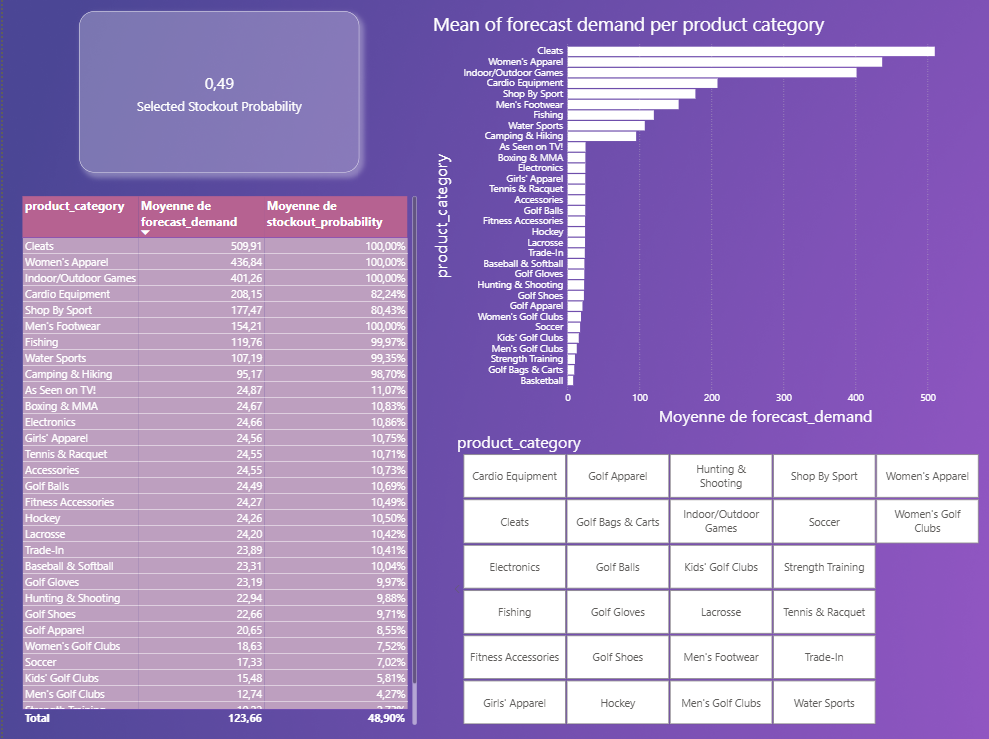
\includegraphics[width=\textwidth]{pbi_forecast_page.png}
   \caption{New Power BI page “Demand Forecast \& Risk” showing forecast and stockout risk visuals.}
   \label{fig:pbi_forecast_page}
\end{figure}

\begin{itemize}
   \item Open the existing Power BI file (\texttt{supply\_chain.pbix}).
   \item Import the \texttt{demand\_forecast} table from PostgreSQL.
   \item Create a new page “Demand Forecast \& Risk” with:
   \begin{itemize}
      \item Table showing average forecast demand and average stockout probability per product category.
      \item Bar chart of forecast demand by category.
      \item Slicer for product category.
      \item Card showing stockout probability for the selected category (using a measure \texttt{AVERAGE(demand\_forecast[stockout\_probability])}).
   \end{itemize}
   \item Save and commit the updated \texttt{.pbix} file.
\end{itemize}

\section{Result}
The \texttt{demand\_forecast} table provides weekly demand forecasts and stockout risks for each product category. The Power BI dashboard now includes predictive analytics, enabling proactive inventory management.





\chapter{Conclusion, Perspectives and code availability}

\section{Summary}
This project built a complete data pipeline for the DataCo SMART SUPPLY CHAIN dataset. Starting from raw CSV files, we performed exploratory data analysis to understand the grain, data quality, and relationships. The EDA directly guided cleaning decisions and the design of a normalised relational model (3NF) with seven tables.

Using PySpark, we implemented cleaning and splitting scripts, producing Parquet files that were loaded into PostgreSQL. The database was validated with integrity checks and optimised with indexes.

Interactive dashboards were created in Power BI, covering sales, logistics, customer segmentation, and product profitability. Finally, we developed a demand forecasting model using XGBoost and quantified stockout risk through Monte Carlo simulation. The forecast results were integrated back into Power BI, enabling predictive analytics.

All work was versioned using Git with a structured branch workflow and pull requests, ensuring collaboration and reproducibility.

\section{Limitations and Future Work}
The dataset is relatively small, so the benefits of distributed processing were not fully exploited. The Monte Carlo simulation assumed a normal distribution of forecast errors; other distributions might be more accurate. The Power BI dashboard is currently static (Import mode); a live connection could be used for real‑time updates.

Future improvements include deploying the pipeline on a cloud platform, adding more features for XGBoost (e.g., holiday indicators), integrating the clickstream logs, and creating a mobile dashboard for supply chain managers.


\section*{Code Availability}
All source code, SQL scripts, and the Power BI dashboard are available in the project’s Git repository:  
\url{https://github.com/onsaissa4/Supply-Chain-Analysis}

\end{document}